\documentclass[10pt,a4paper,onecolumn]{article}
\usepackage{marginnote}
\usepackage{graphicx}
\usepackage{xcolor}
\usepackage{authblk,etoolbox}
\usepackage{titlesec}
\usepackage{calc}
\usepackage{tikz}
\usepackage{hyperref}
\hypersetup{colorlinks,breaklinks,
            urlcolor=[rgb]{0.0, 0.5, 1.0},
            linkcolor=[rgb]{0.0, 0.5, 1.0}}
\usepackage{caption}
\usepackage{tcolorbox}
\usepackage{amssymb,amsmath}
\usepackage{ifxetex,ifluatex}
\usepackage{seqsplit}
\usepackage{fixltx2e} % provides \textsubscript
\usepackage[
  backend=biber,
%  style=alphabetic,
%  citestyle=numeric
]{biblatex}
\bibliography{paper.bib}



% --- Page layout -------------------------------------------------------------
\usepackage[top=3.5cm, bottom=3cm, right=1.5cm, left=1.0cm,
            headheight=2.2cm, reversemp, includemp, marginparwidth=4.5cm]{geometry}

% --- Default font ------------------------------------------------------------
% \renewcommand\familydefault{\sfdefault}

% --- Style -------------------------------------------------------------------
\renewcommand{\bibfont}{\small \sffamily}
\renewcommand{\captionfont}{\small\sffamily}
\renewcommand{\captionlabelfont}{\bfseries}

% --- Section/SubSection/SubSubSection ----------------------------------------
\titleformat{\section}
  {\normalfont\sffamily\Large\bfseries}
  {}{0pt}{}
\titleformat{\subsection}
  {\normalfont\sffamily\large\bfseries}
  {}{0pt}{}
\titleformat{\subsubsection}
  {\normalfont\sffamily\bfseries}
  {}{0pt}{}
\titleformat*{\paragraph}
  {\sffamily\normalsize}


% --- Header / Footer ---------------------------------------------------------
\usepackage{fancyhdr}
\pagestyle{fancy}
\fancyhf{}
%\renewcommand{\headrulewidth}{0.50pt}
\renewcommand{\headrulewidth}{0pt}
\fancyhead[L]{\hspace{-0.75cm}\includegraphics[width=5.5cm]{/Users/Jamie/Library/Caches/org.R-project.R/R/renv/cache/v5/macos/R-4.5/aarch64-apple-darwin20/rticles/0.27/1a05d2cc06f9fb360d2dc15f99293dfe/rticles/rmarkdown/templates/joss/resources/JOSS-logo.png}}
\fancyhead[C]{}
\fancyhead[R]{}
\renewcommand{\footrulewidth}{0.25pt}

\fancyfoot[L]{\footnotesize{\sffamily , (). SemanticDistance: An R
package for Computing Semantic Distance in Structured Texts and
Visualizing Clustering Properties in Unstructured Word
Lists. \textit{Journal of Open Source Software}, (), . \href{https://doi.org/}{https://doi.org/}}}


\fancyfoot[R]{\sffamily \thepage}
\makeatletter
\let\ps@plain\ps@fancy
\fancyheadoffset[L]{4.5cm}
\fancyfootoffset[L]{4.5cm}

% --- Macros ---------

\definecolor{linky}{rgb}{0.0, 0.5, 1.0}

\newtcolorbox{repobox}
   {colback=red, colframe=red!75!black,
     boxrule=0.5pt, arc=2pt, left=6pt, right=6pt, top=3pt, bottom=3pt}

\newcommand{\ExternalLink}{%
   \tikz[x=1.2ex, y=1.2ex, baseline=-0.05ex]{%
       \begin{scope}[x=1ex, y=1ex]
           \clip (-0.1,-0.1)
               --++ (-0, 1.2)
               --++ (0.6, 0)
               --++ (0, -0.6)
               --++ (0.6, 0)
               --++ (0, -1);
           \path[draw,
               line width = 0.5,
               rounded corners=0.5]
               (0,0) rectangle (1,1);
       \end{scope}
       \path[draw, line width = 0.5] (0.5, 0.5)
           -- (1, 1);
       \path[draw, line width = 0.5] (0.6, 1)
           -- (1, 1) -- (1, 0.6);
       }
   }

% --- Title / Authors ---------------------------------------------------------
% patch \maketitle so that it doesn't center
\patchcmd{\@maketitle}{center}{flushleft}{}{}
\patchcmd{\@maketitle}{center}{flushleft}{}{}
% patch \maketitle so that the font size for the title is normal
\patchcmd{\@maketitle}{\LARGE}{\LARGE\sffamily}{}{}
% patch the patch by authblk so that the author block is flush left
\def\maketitle{{%
  \renewenvironment{tabular}[2][]
    {\begin{flushleft}}
    {\end{flushleft}}
  \AB@maketitle}}
\makeatletter
\renewcommand\AB@affilsepx{ \protect\Affilfont}
%\renewcommand\AB@affilnote[1]{{\bfseries #1}\hspace{2pt}}
\renewcommand\AB@affilnote[1]{{\bfseries #1}\hspace{3pt}}
\makeatother
\renewcommand\Authfont{\sffamily\bfseries}
\renewcommand\Affilfont{\sffamily\small\mdseries}
\setlength{\affilsep}{1em}


\ifnum 0\ifxetex 1\fi\ifluatex 1\fi=0 % if pdftex
  \usepackage[T1]{fontenc}
  \usepackage[utf8]{inputenc}

\else % if luatex or xelatex
  \ifxetex
    \usepackage{mathspec}
  \else
    \usepackage{fontspec}
  \fi
  \defaultfontfeatures{Ligatures=TeX,Scale=MatchLowercase}

\fi
% use upquote if available, for straight quotes in verbatim environments
\IfFileExists{upquote.sty}{\usepackage{upquote}}{}
% use microtype if available
\IfFileExists{microtype.sty}{%
\usepackage{microtype}
\UseMicrotypeSet[protrusion]{basicmath} % disable protrusion for tt fonts
}{}

\usepackage{hyperref}
\hypersetup{unicode=true,
            pdftitle={SemanticDistance: An R package for Computing Semantic Distance in Structured Texts and Visualizing Clustering Properties in Unstructured Word Lists},
            pdfborder={0 0 0},
            breaklinks=true}
\urlstyle{same}  % don't use monospace font for urls
\usepackage{graphicx,grffile}
\makeatletter
\def\maxwidth{\ifdim\Gin@nat@width>\linewidth\linewidth\else\Gin@nat@width\fi}
\def\maxheight{\ifdim\Gin@nat@height>\textheight\textheight\else\Gin@nat@height\fi}
\makeatother
% Scale images if necessary, so that they will not overflow the page
% margins by default, and it is still possible to overwrite the defaults
% using explicit options in \includegraphics[width, height, ...]{}
\setkeys{Gin}{width=\maxwidth,height=\maxheight,keepaspectratio}
\IfFileExists{parskip.sty}{%
\usepackage{parskip}
}{% else
\setlength{\parindent}{0pt}
\setlength{\parskip}{6pt plus 2pt minus 1pt}
}
\setlength{\emergencystretch}{3em}  % prevent overfull lines
\setcounter{secnumdepth}{0}
% Redefines (sub)paragraphs to behave more like sections
\ifx\paragraph\undefined\else
\let\oldparagraph\paragraph
\renewcommand{\paragraph}[1]{\oldparagraph{#1}\mbox{}}
\fi
\ifx\subparagraph\undefined\else
\let\oldsubparagraph\subparagraph
\renewcommand{\subparagraph}[1]{\oldsubparagraph{#1}\mbox{}}
\fi


% tightlist command for lists without linebreak
\providecommand{\tightlist}{%
  \setlength{\itemsep}{0pt}\setlength{\parskip}{0pt}}


% Pandoc citation processing
%From Pandoc 3.1.8
% definitions for citeproc citations
\NewDocumentCommand\citeproctext{}{}
\NewDocumentCommand\citeproc{mm}{%
  \begingroup\def\citeproctext{#2}\cite{#1}\endgroup}
\makeatletter
 % allow citations to break across lines
 \let\@cite@ofmt\@firstofone
 % avoid brackets around text for \cite:
 \def\@biblabel#1{}
 \def\@cite#1#2{{#1\if@tempswa , #2\fi}}
\makeatother
\newlength{\cslhangindent}
\setlength{\cslhangindent}{1.5em}
\newlength{\csllabelwidth}
\setlength{\csllabelwidth}{3em}
\newenvironment{CSLReferences}[2] % #1 hanging-indent, #2 entry-spacing
 {\begin{list}{}{%
  \setlength{\itemindent}{0pt}
  \setlength{\leftmargin}{0pt}
  \setlength{\parsep}{0pt}
  % turn on hanging indent if param 1 is 1
  \ifodd #1
   \setlength{\leftmargin}{\cslhangindent}
   \setlength{\itemindent}{-1\cslhangindent}
  \fi
  % set entry spacing
  \setlength{\itemsep}{#2\baselineskip}}}
 {\end{list}}
\usepackage{calc}
\newcommand{\CSLBlock}[1]{#1\hfill\break}
\newcommand{\CSLLeftMargin}[1]{\parbox[t]{\csllabelwidth}{#1}}
\newcommand{\CSLRightInline}[1]{\parbox[t]{\linewidth - \csllabelwidth}{#1}\break}
\newcommand{\CSLIndent}[1]{\hspace{\cslhangindent}#1}



\title{SemanticDistance: An R package for Computing Semantic Distance in
Structured Texts and Visualizing Clustering Properties in Unstructured
Word Lists}

        \author[1, 2]{Jamie Reilly}
          \author[3, 4]{Emily B. Myers}
          \author[4]{Hannah Mechtenberg}
          \author[5, 6, 7]{Jonathan E. Peelle}
    
      \affil[1]{Department of Communication Sciences and Disorders,
Temple University, United States}
      \affil[2]{Department of Psychology and Neuroscience, Temple
University, United States}
      \affil[3]{Department of Speech, Language, and Hearing Sciences,
University of Connecticut, United States}
      \affil[4]{Department of Psychological Sciences, University of
Connecticut, United States}
      \affil[5]{Institute for Cognitive and Brain Health, Northeastern
University, United States}
      \affil[6]{Department of Communication Sciences and Disorders,
Northeastern University, United States}
      \affil[7]{Department of Psychology, Northeastern University,
United States}
  \date{\vspace{-5ex}}

\begin{document}
\maketitle

\marginpar{
  %\hrule
  \sffamily\small

  {\bfseries DOI:} \href{https://doi.org/}{\color{linky}{}}

  \vspace{2mm}

  {\bfseries Software}
  \begin{itemize}
    \setlength\itemsep{0em}
    \item \href{}{\color{linky}{Review}} \ExternalLink
    \item \href{}{\color{linky}{Repository}} \ExternalLink
    \item \href{}{\color{linky}{Archive}} \ExternalLink
  \end{itemize}

  \vspace{2mm}

  {\bfseries Submitted:} \\
  {\bfseries Published:} 

  \vspace{2mm}
  {\bfseries License}\\
  Authors of papers retain copyright and release the work under a Creative Commons Attribution 4.0 International License (\href{http://creativecommons.org/licenses/by/4.0/}{\color{linky}{CC-BY}}).
}

\section{Summary}\label{summary}

\texttt{SemanticDistance} computes pairwise distance between units of
language (e.g., word-to-word, ngram-to-word, turn-to-turn) in both
structured language samples and unstructured word lists.
\texttt{SemanticDistance} has cleaning and formatting options including
stopword removal and lemmatization. The package computes two
complementary cosine distance indices for each pairwise contrast of
interest. \texttt{SemanticDistance} can also be used to examine
clustering properties within unstructured word lists, generating
dendrograms and simple igraph network plots.

\section{Software Design}\label{software-design}

\texttt{SemanticDistance} was is an open-source R package designed to
accommodate a wide range of user expertise (e.g., neuroscience,
linguistics, computer science). The software does not leverage
artificial intelligence or use any proprietary dependencies. The package
instead indexes an internal lookup database containing publicly
available lexical norms.

\section{Statment of need}\label{statment-of-need}

\texttt{SemanticDistance} is unique in its capacity to compute semantic
distance metrics within running language samples (e.g., word-to-word,
bigram-to-word) and to produce semantic network visualizations. The
package also provides complementary (but different) semantic distance
metrics (experiential vs.~embedding) computed over the same stimuli.
This package will support novel insights into the flow of meaning within
naturalistic language samples.

\section{Research Impact Statement}\label{research-impact-statement}

\texttt{SemanticDistance} has supported one peer-reviewed publication to
date in the journal, \texttt{Cortex} (Mechtenberg et al. 2026) along
with one refereed conference presentation at the annual conference of
the Society for the Neurobiology of Language. Importantly, the
application enables a variety of analyses that have been formerly
difficult or impossible, including comparing semantic distance measures
with other measure of prediction in language, including those generated
by large language models.

\section{Description}\label{description}

\texttt{SemanticDistance} bundles text cleaning and formatting options
(e.g., stopword removal, lemmatization) with two two complementary
semantic distance metrics (i.e., experiential vs.~embeddings) that
characterize/quantify similarity between pairs of language constituents
(e.g., words, ngrams, turns). Semantic distance values are derived on
demand by indexing two large lookup databases that contain semantic
vectors for many English words.\newline   

One of the most innovative functions of \texttt{SemanticDistance} is its
capacity to generate rolling measures of semantic distance within
stories or narratives with chunk sizes (e.g., word-to-word,
turn-to-turn). Chunk size is an optional argument for many of the
software's functions. For example, if a user specified a chunk or n-gram
size of 5 words, the software would automatically compute a rollinhg
measure of semantic distance betweem each new word in a language sample
relative to the five words that preceded it. Figure 1 illustrates
options for computing rolling semantic distance in text samples word
order is essential (e.g., monologues, dialogues, narratives). Figure 2
represents options for computing distances in list formats (e.g., word
pairs in columns, unordered lists). \newline  

\begin{figure}
\centering
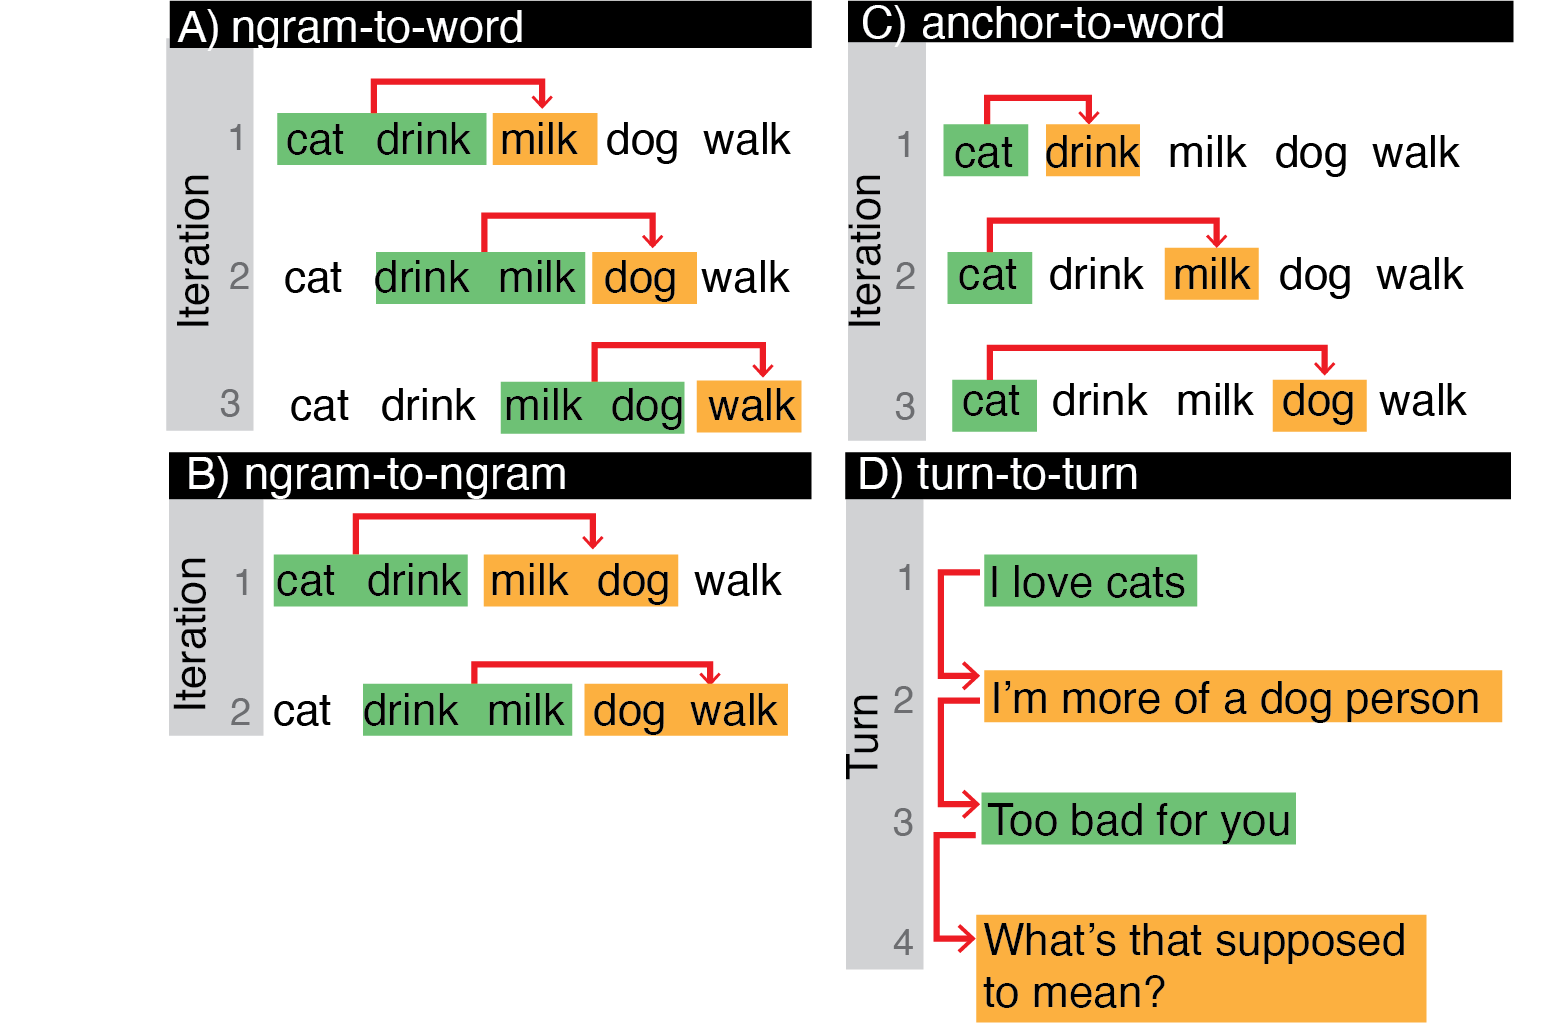
\includegraphics[width=0.7\linewidth,height=\textheight,keepaspectratio,alt={Figure 1: Options for ordered text formats}]{Fig1_OrderedText.png}
\caption{Figure 1: Options for ordered text formats\label{fig:demo}}
\end{figure}

\vspace*{-0.5cm}

\newline

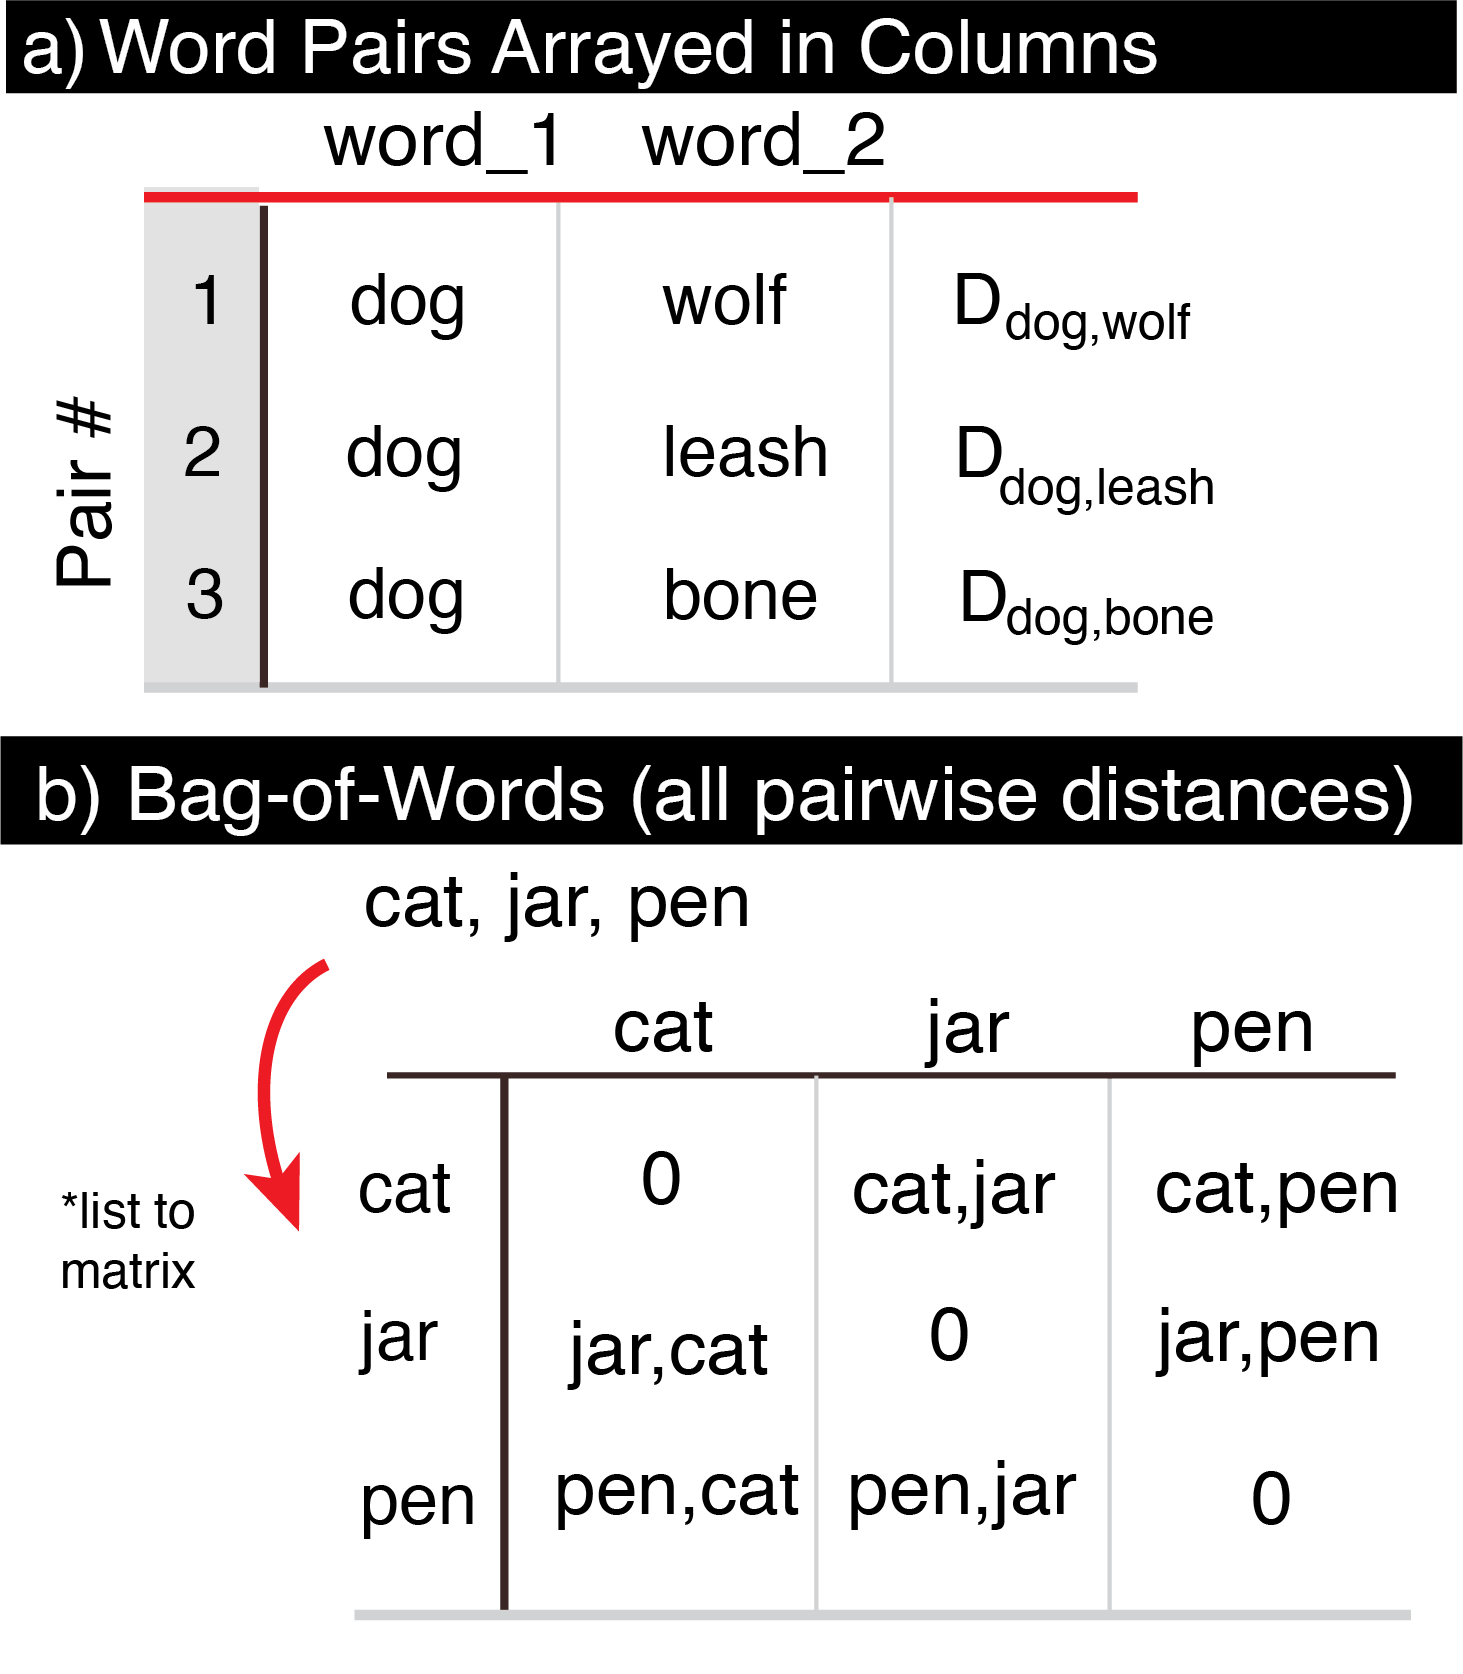
\includegraphics[width=0.3\linewidth,height=\textheight,keepaspectratio,alt={Figure 2: Options for unordered lists}]{Fig2_UnorderedLists.png}
\vspace*{-0.5cm} \newline

\section{AI Usage}\label{ai-usage}

\texttt{SemanticDistance} uses an internal database composed of many
words with a fixed set of embeddings. The software does not use AI or
rely on proprietary package dependencies. We did use GPT-4.0 (OpenAI) to
troubleshoot R coding errors and assist with generating complex regular
expressions (regex) used for cleaning text data.

\section*{References}\label{references}
\addcontentsline{toc}{section}{References}

\protect\phantomsection\label{refs}
\begin{CSLReferences}{1}{0}
\bibitem[\citeproctext]{ref-Mechtenberg:2026}
Mechtenberg, Hannah, Jamie Reilly, Jonathan E. Peelle, and Emily B.
Myers. 2026. {``Measuring Brain Sensitivity to Semantic Distance in
Spoken Narrative Comprehension.''} \emph{Cortex} 195 (February): 28--42.
\url{https://doi.org/10.1016/j.cortex.2025.12.004}.

\end{CSLReferences}

\end{document}
